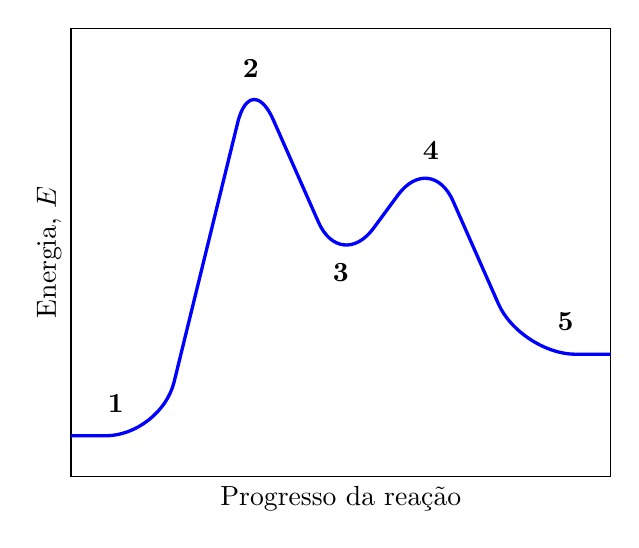
\begin{tikzpicture}
         \begin{axis}
             [
                 ylabel = {Energia, $E$},
                 xlabel = {Progresso da reação},
                 xmin =  0,   xmax = 6,
                 ymin = -0.5, ymax = 5,
                 xtick = \empty,
                 ytick = \empty,
             ]
         \draw [draw=blue, very thick, rounded corners=2em]
             (axis cs: 0.0, 0.0) -- 
             (axis cs: 1.0, 0.0) -- 
             (axis cs: 2.0, 4.5) -- 
             (axis cs: 3.0, 2.0) --
             (axis cs: 4.0, 3.5) --
             (axis cs: 5.0, 1.0) --
             (axis cs: 6.0, 1.0);
         \node at (axis cs: 0.5, 0.4) {\textbf{1}};
         \node at (axis cs: 2.0, 4.5) {\textbf{2}};
         \node at (axis cs: 3.0, 2.0) {\textbf{3}};
         \node at (axis cs: 4.0, 3.5) {\textbf{4}};
         \node at (axis cs: 5.5, 1.4) {\textbf{5}};
          \end{axis}
      \end{tikzpicture}